\chapter{Intro}

\pagenumbering{arabic}
\section{Introducción}
\begin{center}
	En este capítulo se presenta una introducción a las formas\\ 		
	cuadráticas, sus representaciones y su clasificación. Esto\\ 
	con el fin permitir al lector un mejor entendimiento del\\
	problema que se plantea en este trabajo de tesis.
\end{center}

\subsection{FORMAS CUADRÁTICAS}
\paragraph*{}
Esta sección fue adaptada de Lay (2001). Algunas demostraciones aquí omitidas pueden consultarse en dicha referencia.

\paragraph*{}
Fijamos un conjunto de variables $\{x_1, x_2, \ldots, x_n\}$. Un \textbf{monomio} es un producto de la forma $x_{1}^{e_{1}} \cdot x_{2}^{e_{2}} \cdots x_{n}^{e_{n}}$ donde cada $e_{i}$ es un número natural. Un término se forma al multiplicar a un monomio por una constante, a la cual llamamos \textbf{coeficiente} del término. Un \textbf{polinomio} es una suma finita de términos.

\paragraph*{}
Ejemplo: $7x^{2}y + 5x^z{4} - y$ es un polinomio sobre las variables $x$, $y$ y $z$ con tres monomios: $x^{2}y$, $xz^{4}$ y $y$ cuyos respectivos coeficientes son 2, 4, 1 respectivamente.

\paragraph*{}
Una \textbf{forma cuadrática} es un polinomio $q : \mathbb{R}^{n} \rightarrow \mathbb{R}$(con $n > 0$) si cada monomio del mismo es una variable al cuadrado o la multiplicación de dos variables. Esto es equivalente a decir que $q$ se puede expresar como

\begin{center}
$$q(x_{1}, x_{2}, \ldots, x_{n}) = \sum_{i=1}^{n} q_{ii}x_{i}^{2}+ \sum_{j=2}^{n}\sum_{i=1}^{j-1} q_{ij}x_{i}x_{j}$$
\end{center}

\paragraph*{}
Los ejemplos más usuales aparecen al lado izquierdo del signo igual de las ecuaciones en las cónicas con centro en el origen

\begin{center}
$$ax^{2} + 2bxy + cy^{2} = d$$
\end{center}

\paragraph*{}
y de las superficies cuadráticas con centro en el origen

\begin{center}
$$ax^{2} + 2dxy + 2exz + by^{2} + 2fyz + cz^{2} = g$$
\end{center}

\paragraph*{}
donde $a$, $b$, $c$, $d$, $e$, $f$ y $g$ son números reales. Este tipo de polinomios surgen de manera natural en diversas áreas de la ingeniería, procesamiento de señales, cinética, economía, geometría diferencial y estadística.

\paragraph*{}
En algunos curso básicos de álgebra lineal se suele definir el concepto de forma cuadrática como una función que se puede escribir como

\begin{center}
$$q(\overrightarrow{x}) = \frac{1}{2} \overrightarrow{x}^{T} A \overrightarrow{x}$$
\end{center}

\paragraph*{}
para alguna matriz simétrica $A$. En realidad esta representación matricial es equivalente a nuestra definición con monomios; a continuación veremos c+omo pasar de una representación a otra. Primero notemos que $\frac{1}{2} \overrightarrow{x}^{T} A \overrightarrow{x}$ se puede reescribir como sigue:

\begin{align*}
\frac{1}{2} \overrightarrow{x}^{T} A \overrightarrow{x} &= \frac{1}{2}[x_{1}, x_{2},\ldots,x_{n}] 
\begin{bmatrix}
a_{11} & a_{12} & \cdots & a_{1n}\\
a_{21} & a_{22} & \cdots & a_{2n}\\
\vdots & \vdots & \ddots & \vdots \\
a_{n1} & a_{n2} & \cdots & a_{nn}
\end{bmatrix} 
\begin{bmatrix}
x_{1}\\
x_{2}\\
\vdots\\
x_{n}
\end{bmatrix} \\ 
&= \frac{1}{2} \left[\sum_{i=1}^{n} a_{i1}x_{i}, \sum_{i=1}^{n} a_{i2}x_{i}, \ldots , \sum_{i=1}^{n} a_{in}x_{i} \right] 
\begin{bmatrix}
x_{1}\\
x_{2}\\
\vdots\\
x_{n}
\end{bmatrix} \\ 
&=   \frac{1}{2} \left[\sum_{i=1}^{n} a_{i1}x_{i}x_{1} + \cdots + \sum_{i=1}^{n} a_{in}x_{i}x_{n}\right]\\ 
&=   \frac{1}{2} \sum_{i=1}^{n}\sum_{j=1}^{n} a_{ij}x_{i}x_{n}
\end{align*}


\paragraph*{}
Al desarrollar esta suma se puede ver que el coeficiente de $x_{i}$ $x_{j}$ es $q_{ij} = \frac{1}{2} \left(a_{ij} + a_{ji} \right)$ porque $x_{i}$ $x_{j}$ = $x_{i}$ $x_{j}$, pero como dijimos que $A$ es simétrica $\left( a_{ij} = a_{ji}\right)$ entonces $q_{ij} = a_{ij}$. En particular cuando $i = j$ se tiene que el coeficiente de $x_{i}^{2}$ es $q_{ii} = \frac{1}{2}a_{ii}$. Por lo tanto tenemos la siguiente identidad:


\begin{equation}\tag{1.1}
    \frac{1}{2} \overrightarrow{x}^{T} A \overrightarrow{x} = \sum_{i=1}^{n}\frac{1}{2} a_{ii}x_{i}^{2} + \sum_{j=2}^{n}\sum_{i=1}^{j-1} a_{ij}x_{i}x_{j}
\end{equation}

\paragraph*{}
La matriz simétrica $A$ de esta identidad se conoce como \textbf{matriz asociada a la forma cuadrática $q$}. Nosotros la vamos a denotar por $A_{q}$, y según la ecuación 1.1 se puede calcular como sigue:

\begin{equation}\tag{1.2}
a_{ij} = \left \{ 
    \begin{matrix} 
    q_{ij} & \mbox{si } i < j\\
    2q_{ij} & \mbox{si } i = j\\ 
    q_{ji} & \mbox{si } i > j
    \end{matrix}\right. 
\end{equation}

\paragraph*{}
Por ejemplo, para $q(x, y, x) = 3x^{2} + 3xy + 16xz - 4y^{2} + 4z^{2} + 6yz$

\begin{equation*}
q(x. y. z) = = \frac{1}{2}\left[x ~  y ~ z\right] 
\begin{bmatrix}
3 & 1 & 9\\
2 & 4 & 6\\
7 & 0 & 4
\end{bmatrix}
\begin{bmatrix}
x\\
y\\
z\\
\end{bmatrix}
\end{equation*}

\paragraph*{}
\textbf{CAMBIO DE VARIABLE}

\paragraph*{}
Un \textbf{cambio de variable} es una ecuación de la forma

\begin{equation}\tag{1.3}
    \begin{matrix} 
    \overrightarrow{x} = P\overrightarrow{y} & \mbox{o bien } & \overrightarrow{y} = P^{-1}\overrightarrow{x}\\
    \end{matrix}. 
\end{equation}

\paragraph*{}
donde $P$ es una matriz invertible y $\overrightarrow{y}$ es un nuevo vector variable en $\mathrm{R}^{n}$. Si se aplica el cambio de variable (1.3) sobre una forma cuadrática $q(\overrightarrow{x}) = \frac{1}{2}\overrightarrow{x}^{T}A\overrightarrow{x}$ se obitene una matriz cuadrática $q'(\overrightarrow{y})$ cuya matriz asociada es $P^{T} ~ A ~ P$:

\begin{equation*}
    \frac{1}{2}\overrightarrow{x}^{T}\overrightarrow{x} = \frac{1}{2}\left(P\overrightarrow{y}\right)^{T}~A~\left(\overrightarrow{y}\right) = \frac{1}{2}\left(\overrightarrow{y}^{T} P^{T}\right)~A~\left(P\overrightarrow{y}\right) = \frac{1}{2}\overrightarrow{y}^{T}\left(P^{T}~A~P\right)\overrightarrow{y}
\end{equation*}.

\paragraph*{}
Gatantizamos que $P^{T}~A~P$ es una matriz simétrica (y por tanto que en verdad corresponde a otra forma cuadrática) porque

\begin{eqnarray*}
(P^{T}~A~P)^{T}&=&P^{T}~A^{T}~\left(P^{T}\right)^{T}\\
&=&P^{T}~A^{T}~P\\
&=&P^{T}~A~P
\end{eqnarray*}

\paragraph*{}
Mediante el cambio de variable $\overrightarrow{y} = P~\overrightarrow{x}$ tenemos que $q(\overrightarrow{x}) = q'(\overrightarrow{y})$ y diremos que $q$ y $q'$ son \textbf{equivalentes} mediante la matriz invertible $P$. Si denotamos $\overrightarrow{y} = L(\overrightarrow{x})$(es decir, $L(\overrightarrow{x}) = P(\overrightarrow{x}))$ entonces $q'(\overrightarrow{y}) = q'\left(L(\overrightarrow{x})\right) = \left(q' \circ L\right)(\overrightarrow{x})$, por lo tanto
$$q' = q \circ L$$

\paragraph*{}
Vale la pena notar algunas cosas sobre este ejemplo:
\begin{itemize}
    \item $P$ resultó ser una \textbf{matriz ortogonal}, en otras palabras, $P^{-1} = P^{T}$.
    \item $A$ es una matriz \textbf{ortogonalmente diagonizable}, en otras palabras, existe una matriz ortogonal $P$ tal que $P^{-1}~A~P$ es una matriz diagonal.
\end{itemize}

\begin{theorem}
Toda matriz es ortogonalmente diagonizable si y solo si es simétrica
\end{theorem}

\paragraph*{}
Este teorema se dejara sin demostración. Lo importante es que, a partir de este teorema, y dado que las matrices asociadas a las formas cuadráticas son simëtricas, se sigue el siguente resultado:

\begin{theorem}
Toda forma cuadrática $q(\overrightarrow{x})$ es equivalente a una matriz ortogonal $P$ a una forma cuadrática 
\begin{equation}
    q'(\overrightarrow{y}) = \lambda_{1}y_{1}^{2} + \lambda_{2}y_{2}^{2} + \cdots + \lambda_{n}y_{n}^{2}
\end{equation}
\end{theorem}

\begin{proof}
La matriz $A$ asociada a $q$ es simétrica, luego por teorema anterior existe una matriz $P$ tal que 
\begin{equation*}
    P^{-1}~A~P = \begin{bmatrix}
    \lambda_{1} & &\\
    & \ddots & \\
    & & \lambda_{n}
    \end{bmatrix}
\end{equation*}

Haciendo $\overrightarrow{x} = P\overrightarrow{y}$ y se obtiene $q'(\overrightarrow{y}) = \frac{1}{2}\overrightarrow{y}^{T}\left(P^{T}~A~P\right)\overrightarrow{y} = \lambda_{1}y_{1}^{2} + \lambda_{2}y_{2}^{2} + \cdots + \lambda_{n}y_{n}^{2}$

\end{proof}

\paragraph*{}
Como se vera, esta representación es extremadamente útil para clasificar formas cuadráticas. Diremos que nuna forma cuadrática $q$ es \textbf{definida positiva} si $q(\overrightarrow{x}) > 0, ~\forall~ \overrightarrow{x} \neq \overrightarrow{0}$ 

\begin{lemma}
Si dos formas cuadráticas $q(\overrightarrow{x})$ y $q'(\overrightarrow{y})$ son equivalentes mediante el cabio ded variable $\overrightarrow{y} = P\overrightarrow{x}$ y si una de ellas es definada positiva entonces la otra también.
\end{lemma}

\begin{proof}
Supongamos que $q(\overrightarrow{x})$ es definida positiva y defínase la transformación lineal $L(\overrightarrow{x}) = P\overrightarrow{x}$, entonces $L(\overrightarrow{0}) = L(\overrightarrow{0}+ \overrightarrow{0}) = L(\overrightarrow{0}) + L(\overrightarrow{0})$, de donde $L(\overrightarrow{0}) = \overrightarrow{0}$. Como $P$ es una matriz invertible entonces $L^{-1}(\overrightarrow{x}) = P^{-1}x$. En particular $L$ debe ser inyectiva y por lo tanto $L(\overrightarrow{x})=\overrightarrow{0}$ implica que $\overrightarrow{x}=\overrightarrow{0}$. SI $q$ es definida positiva entonces $q(\overrightarrow{x}) = q'(\overrightarrow{y}) > 0$ para todo $\overrightarrow{x} = \overrightarrow{0}$; por lo tanto $q'$ es definida positiva , entonces aplicando el mismo razonamiento con $L(\overrightarrow{y}) = P^{-1}\overrightarrow{y}$ se llega a la conclusión de que $q$ tambien es definida positiva. 
\end{proof}

\begin{theorem}
Sea $q$ una forma cuadrática y supongamos que 
\begin{equation*}
q \left(\overrightarrow{x}\right) = q'(y) = \lambda_{1}y_{1}^{2} + \lambda_{2}y_{2}^{2} + \cdots + \lambda_{n}y_{n}^{2}
\end{equation*}
entonces $q$ es definida positiva si y solo si todos los $\lambda_{i} > 0$ 
\end{theorem}

\begin{proof}
Por el lema anterior $q$ es definida positiva si y solo si $q'$ es definida positiva. Por contradicción, si $\lambda_{i} \leq 0$ entonces definimos $y' = (y_{1}, y_{2}, \ldots, y_{n})$ donde todos los $y_{k}=0$ excepto $y_{i} = 1$. Claramente $\overrightarrow{y} \neq \overrightarrow{0}$ pero $q(\overrightarrow{y}) = \lambda_{i} \leq 0$; por lo tanto $q$ no es definida positiva.
\end{proof}

\paragraph{}
Como las forma  cuadráticas se pueden representar mediante matrices entonces podemos decir que una matriz $A$ es definida positiva si su forma cuadrática asociada $q(\overrightarrow{x}) = \frac{1}{2}\overrightarrow{x}^{T}A\overrightarrow{x}$ es definida positiva.

\paragraph{}
A continuación enunciamos (sin demostración) un teorema típico de
los cursos de análisis numérico que nos da un criterio computacional-
mente eficiente para decidir cuándo una matriz simétrica es definida
positiva:

\begin{theorem}
Una matriz $A$ es definida positiva si y solo si tiene \textbf{factorización de Cholesky}, es decir, se puede escribir como $A=R^{T}R$ donde $R$ es una matriz triangula superior con entradas positivas.
\end{theorem}

\subsection{FORMAS UNITARIAS}
\paragraph*{}
Esta sección fue adaptada de Ringel (1985) y Gabriel \& Rotter (1997).\\
Las \textbf{formas cuadráticas enteras} son un caso especial de las formas cuadráticas donde todos los coeficientes $q_{ij}$ son todos números enteros. Si además exigimos que $q_{ii} = 1$ para $i = 1, 2, \ldots, n$ entonces las llamamos \textbf{formas cuadráticas unitarias}. Dado que en el resto de   

\paragraph*{}
\textbf{CAMBIO DE VARIABLE ENTERO}

\paragraph*{}
Una \textbf{matriz entera} $M$ es una matriz tal que todas sus entradas son números enteros, y es $\mathbb{Z}$\textbf{-invertible} si además su matriz inversa $M^{-1}$ tambien es una matriz entera. Un \textbf{cambio de variable entero} es un cambio de variable $\overrightarrow{y} = P\overrightarrow{x}$ donde $P$ es una matriz $\mathbb{Z}$-invertible. Los cambios de variables enteros tienen la propiedad de que transforman formas cuadráticas enteras en formas cuadráticas enteras(demostración: sean $A$ y $P$ matrices enteras, entonces $P^{T}AP$ es una matriz entera). Cuando $q(\overrightarrow{x}) = q'(\overrightarrow{y})$ mediante el cambio de variable entero $\overrightarrow{y} = P\overrightarrow{x}$ diremos que $q$ y $q'$ son $\mathbb{Z}$-\textbf{equivalentes} mediante la matriz $\mathbb{Z}$-invertible $P$.

\paragraph*{}
\textbf{GRÁFICAS DE DYNKIN}

\paragraph*{}
Si $q$ es una forma unitaria entonces le asociaremos una multigráfica \textbf{$B$}$_{q}$ construida de la siguiente manera:

\begin{itemize}
    \item Existe un vértice $x_{i}$ para cada variable $x_{1}$
    \item Si $q_{ij} > 0$ entonces hay $q_{ij}$ aristas punteadas entre los vértices $x_{i}$ y $x_{j}$(cada una de ellas denotada como $x_{i}$ - - - - $x_{j}$)
    \item Si $q_{ij} < 0$ entonces hay $|q_{ij}|$ aristas sólidas entre los vértices $x_{i}$ y $x_{j}$(cada una de ellas denotada por $x_{i} \rule[1mm]{5mm}{0.1mm} x_{j}$)
\end{itemize}

\begin{center}
 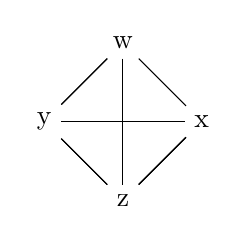
\begin{tikzpicture}
  \node (v0) at (1, 0.) {x};
  \node (v1) at (-1, 0) {y};
  \node (v2) at (0, -1) {z};
  \node (v3) at (0, 1) {w};
  \draw (v0) -- (v1);
  \draw (v0) -- (v2);
  \draw (v1) -- (v0);
  \draw (v1) -- (v2);
  \draw (v1) -- (v3);
  \draw (v2) -- (v1);
  \draw (v2) -- (v0);
  \draw (v2) -- (v3);
  \draw (v3) -- (v2);
  \draw (v3) -- (v1);
  \draw (v3) -- (v0);
\end{tikzpicture}
\end{center}

\paragraph*{}
Claramente podemos revertir este proceso y asociar toda gráfica $G$ (posiblemente aristas punteadas) una forma unitaria que denotaremos por \textbf{$q_{G}$}. Ahora, toda la información de $q_{G}$ está codificada en $G$. La existencia de un vértice $x$ nos dice la forma cuadrática está definida sobre alguna variable $x$ y que contiene el término $x^{2}$ (porque $q$ es una forma cuadrática unitaria). El coeficiente del monomio $xy$ es $c = a_{p} - a_{s}$ donde $a_{p}$ es la cantidad de aristas punteadas enter $x$ y $y$, y $a_{s}$ es la cantidad de aristas sólidas entre estos mismos vértices. Más aún cabe recalcar que nosotros estamos descartando gráficas con lazos, por lo que cualquier gráfica en verdad define a una forma cuadrática unitaria.\\

\paragraph*{}
Decimos que la forma unitaria cuadrática $q$ es \textbf{positiva} si es definida positiva.

\begin{theorem}
Toda forma unitaria $q$ es definida positiva si y solamente si $q$ es $\mathbb{Z}$-equivalente a otra forma unitaria $q'$ donde cada componente conexa de $\textbf{B}_{q'}$ es una gráfica de Dynkin.
\end{theorem}

\begin{table}[]
    \centering
    \begin{tabular}{ll}
    \hline
    Notación \vline & Gráfica\\ 
    \hline
    $\DynA_{n}$, $n\ge1$ &
    \begin{tikzpicture}
    [baseline=(v1.base)]
    \node (v1) at (0, 0) {$1$};
    \node (v2) at (1, 0) {$2$};
    \node (v3) at (4, 0) {$n$};
    \node[draw = none] (v5) at (2.5, 0) {$\ldots$};
    \draw (v1) -- (v2) -- (2, 0);
    \draw (3, 0) -- (v3);
    \end{tikzpicture}\\
    \newline
    $\DynD_{n}$, $n\ge4$ &
    \begin{tikzpicture}
    [baseline=(v1.base)]
    \node (v1) at (0, 0) {$2$};
    \node (v2) at (1, 0) {$3$};
    \node (v3) at (2, 0) {$4$};
    \node (v4) at (5, 0) {$n$};
    \node (v5) at (1, 1) {$1$};
    \node[draw = none] (dots) at (3.5, 0) {$\ldots$};
    \draw (v1) -- (v2) -- (v3) -- (3, 0); \draw (v5)
    -- (v2); \draw (4, 0) -- (v4);
    \end{tikzpicture} \\
    \newline
    $\DynE_{n}$, $n=6$ &
    \begin{tikzpicture} [baseline=(v1.base)]
    \node (v1) at (0, 0) {$2$};
    \node (v2) at (1, 0) {$3$};
    \node (v3) at (2, 0) {$4$};
    \node (v4) at (3, 0) {$5$};
    \node (v5) at (4, 0) {$6$};
    \node (v6) at (2, 1) {$1$};
    \draw (v1) -- (v2) -- (v3) -- (v4);
    \draw (v6) -- (v3);
    \draw (v5) -- (v4);
    \end{tikzpicture}\\
    \newline
    $\DynE_{n}$, $n=7$ &
    \begin{tikzpicture} [baseline=(v1.base)]
    \node (v1) at (0, 0) {$2$};
    \node (v2) at (1, 0) {$3$};
    \node (v3) at (2, 0) {$4$};
    \node (v4) at (3, 0) {$5$};
    \node (v5) at (4, 0) {$6$};
    \node (v7) at (5, 0) {$7$};
    \node (v6) at (2, 1) {$1$};
    \draw (v1) -- (v2) -- (v3) -- (v4);
    \draw (v6) -- (v3);
    \draw (v4) -- (v5);
    \draw (v5) -- (v7);
    \draw (v6) -- (v3);
    \end{tikzpicture}\\
    \newline
    $\DynE_{n}$, $n=8$ &
    \begin{tikzpicture} [baseline=(v1.base)]
    \node (v1) at (0, 0) {$2$};
    \node (v2) at (1, 0) {$3$};
    \node (v3) at (2, 0) {$4$};
    \node (v4) at (3, 0) {$5$};
    \node (v5) at (4, 0) {$6$};
    \node (v7) at (5, 0) {$7$};
    \node (v8) at (6, 0) {$8$};
    \node (v6) at (2, 1) {$1$};
    \draw (v1) -- (v2) -- (v3) -- (v4);
    \draw (v6) -- (v3);
    \draw (v4) -- (v5);
    \draw (v5) -- (v7);
    \draw (v7) -- (v8);
    \end{tikzpicture}
    \end{tabular} 
    \caption{Caption}
    \label{tab:my_label}
\end{table}

\paragraph{}
Para poder hacer la demostaración hay que comprender el teorema. El teorema dice que la forma unitaria $q(\overrightarrow{x}) = \frac{1}{2}\overrightarrow{x}^{T}A\overrightarrow{x}$ es positiva si y solo si se puede llevar, mediante un cambio de variable entero $\overrightarrow{y} = P\overrightarrow{x}$, a la forma $q'(\overrightarrow{y}) = \frac{1}{2}\overrightarrow{y}^{T}\left(P^{T}AP\right)\overrightarrow{y}$ donde $\textbf{B}_{q'}$, tiene la propiedad de que cada una de sus componentes conexas es una gráfica de Dynkin. A dicha gráfica $\textbf{B}_{q'}$ se le llama el \textbf{tipo Dynkin} de $q$.

\paragraph{Ejemplo}
La forma unitaria
\begin{equation}
    q(w, x, y, z) = x^{2} + y^{2} + z^{2} + w^{2}
\end{equation}

\paragraph{}
La demostración del teorema 1.5 se divide en dos parts: primero se demuestra que las gráficas de Dynkin son las únicas gráficas conexas de aristas solidas que definen las formas unitarias que son definidas positivas (tomando en cuentra inclusive a las gráficas de aristas múltiples); luego se demuestra que siempre es psible hacer cambios de variable enteros de tal manera que la gráfica resultante no contenga aristas sólidas.

\begin{lemma}
Las gráficas de Dynkin son las únicas gráficas conexas de aristas sólidas que tienen asociadas formas unitarias positivas.
\end{lemma}

\paragraph{}
Para comenzar necesitamos convencernos en verdad de que las gráficas de Dynkin definen formas unitarias positivas. Comencemos con las gráficas de tipo $\DynA_{n}$:

$$x_{1} \rule[1mm]{5mm}{0.1mm} x_{2} \rule[1mm]{5mm}{0.1mm}\cdots\rule[1mm]{5mm}{0.1mm} x_{n}$$

\paragraph{}
Consideremos con la identidad:

\begin{equation*}
    \frac{1}{2}\left(x_{i} - x_{j}\right)^{2} = \frac{1}{2}x_{i}^{2} - x_{i}x_{j} + \frac{1}{2}x_{j}^{2}
\end{equation*}

\paragraph{}
Podemos reescribir la forma unitaria asociada a $\DynA_{n}$ como

\begin{eqnarray*}
 q_{\DynA_{n}}(\overrightarrow{x}) &  =  & \sum_{i=1}^{n}x_{i}^{2} - \sum_{i=1}^{n-1} x_{i}x_{i+1}\\
 &  =  & \frac{1}{2}x_{1}^{2} + \sum_{i=1}^{n-1}\left(\frac{1}{2}x_{i}^{2} + \frac{1}{2} x_{i+1}^{2}\right) + \frac{1}{2}x_{n}^{2} + \sum_{i=1}^{n-1} \left(-x_{i}x_{i+1}\right)\\
 &  =  & \frac{1}{2}x_{1}^{2} + \sum_{i=1}^{n-1}\left(\frac{1}{2}x_{i}^{2} - x_{i}x_{i+1} + \right) + \frac{1}{2}x_{i+1}^{2}\\
 &  =  & \frac{1}{2}x_{i}^{2} + \sum_{i=1}^{n-1}\frac{1}{2}\left(x_{i} - x_{i+1}\right)^{2} + \frac{1}{2}x_{n}^{2}
\end{eqnarray*}

\paragraph{}
Por el teorema 1.3 concluimos que $q_{\DynA_{n}}$ es definida positiva. La demostración para la forma unitaria $q_{\DynD_{n}}$ es similar solo que en este caso se usa la identidad:

\begin{equation*}
    \frac{1}{2}\left[(x_{3} - x_{2} - x_{1})^{2} + (x_{2} - x_{1})^{2}\right] = x_{1}^{2} + x_{2}^{2} + \frac{1}{2}x_{3}^{2} - x_{1}x_{3} - x_{2}x_{3}
\end{equation*}

\paragraph{}
de tal forma que 

\begin{eqnarray*}
 q_{\DynD_{n}}(\overrightarrow{x}) &  =  & \sum_{i=1}^{n}x_{i}^{2} - x_{1}x_{3} -  \sum_{i=1}^{n-1} x_{i}x_{i+1}\\
 &  =  & \frac{1}{2}\left[(x_{3} - x_{2} - x_{1})^{2} + (x_{2} - x_{1})^{2} + \sum_{i=3}^{n-1}(x_{i} - x_{i+1})^{2}  + x_{n}^{2}\right]
\end{eqnarray*}. 

\paragraph{}
Para las gráficas $\DynE_{6}$, $\DynE_{7}$ y $\DynE_{8}$ usaremos el siguente razonamiento: 

\paragraph{}
Supongamos que $A_{\Delta}$ es la matriz asociada a la gráfica $\Delta$ (con $\Delta = \DynE_{6},\DynE_{7},\DynE_{8}$); si existe una matriz $R_{\Delta}$ tal que $A_{\Delta} = R_{\Delta}^{T}R_{\Delta}$ entonces por teorema 1.4 se sigue que $\Delta$ define una forma unitaria definida positiva.

\paragraph{}
En efecto tenemos que:

\begin{eqnarray*}
 A\DynE_{6} &  =  & \begin{bmatrix}
 2 & 0 & 0 & -1 & 0 & 0\\
 0 & 2 & -1 & 0 & 0 & 0\\
 0 & -1 & 2& -1 & 0 & 0\\
 -1 & 0 & -1 & 2 & -1 & 0\\
 0 & 0 & 0 & -1 & 2 & -1\\
 0 & 0 & 0 & 0 & -1 & 2\\
 \end{bmatrix}\\
 R\DynE_{6} &  =  & \begin{bmatrix}
 \sqrt{2} & 0 & 0 & -\frac{1}{\sqrt{2}} & 0 & 0\\
 0 & sqrt(2) & - \frac{1}{\sqrt{2}}& 0 & 0 & 0\\
 0 & 0 & \frac{\sqrt{3}}{\sqrt{2}} & -\frac{\sqrt{2}}{\sqrt{3}} & 0 & 0\\
 0 & 0 & 0 & \frac{\sqrt{5}}{\sqrt{6}} & -\frac{\sqrt{6}}{\sqrt{5}} & 0\\
 0 & 0 & 0 & 0 & \frac{2}{\sqrt{5}} & -\frac{\sqrt{5}}{2}\\
 0 & 0 & 0 & 0 & 0 & \frac{\sqrt{3}}{2}\\
 \end{bmatrix}\\
 \end{eqnarray*}
 
 \begin{eqnarray*}
 A\DynE_{7} &  =  & \begin{bmatrix}
 2 & 0 & 0 & -1 & 0 & 0 & 0\\
 0 & 2 & -1 & 0 & 0 & 0 & 0\\
 0 & -1 & 2 & -1 & 0 & 0 & 0\\
 -1 & 0 & -1 & 2 & -1 & 0 & 0\\
 0 & 0 & 0 & -1 & 2 & -1 & 0\\
 0 & 0 0 & 0 & 0 & -1 & 2 & -1\\
 0 & 0 & 0 & 0 & 0 & -1 & 2\\
 \end{bmatrix}\\
 R\DynE_{7} &  = & \begin{bmatrix}
 \sqrt{2} & 0 & 0 & -\frac{1}{\sqrt{2}} & 0 & 0 & 0 & 0\\
 0 & sqrt(2) & - \frac{1}{\sqrt{2}}& 0 & 0 & 0 & 0 & 0\\
 0 & 0 & \frac{\sqrt{3}}{\sqrt{2}} & -\frac{\sqrt{2}}{\sqrt{3}} & 0 & 0 & 0 & 0\\
 0 & 0 & 0 & \frac{\sqrt{5}}{\sqrt{6}} & -\frac{\sqrt{6}}{\sqrt{5}} & 0 & 0 & 0\\
 0 & 0 & 0 & 0 & \frac{2}{\sqrt{5}} & -\frac{\sqrt{5}}{2} & 0 & 0\\
 0 & 0 & 0 & 0 & 0 & \frac{\sqrt{3}}{2} & -\frac{2}{\sqrt{3}}\\
 0 & 0 & 0 & 0 & 0 & 0 & 0 & \frac{\sqrt{2}}{\sqrt{3}}\\
 \end{bmatrix}\\
 \end{eqnarray*}
 
 \begin{eqnarray*}
 A\DynE_{8} &  =  & \begin{bmatrix}
 2 & 0 & 0 & -1 & 0 & 0 & 0 & 0\\
 0 & 2 & -1 & 0 & 0 & 0 & 0 & 0\\
 0 & -1 & 2 & -1 & 0 & 0 & 0 & 0\\
 -1 & 0 & -1 & 2 & -1 & 0 & 0 & 0\\
 0 & 0 & 0 & -1 & 2 & -1 & 0 & 0 \\
 0 & 0 & 0 & 0 & -1 & 2 & -1 & 0\\
 0 & 0 & 0 & 0 & 0 & -1 & 2 & -1\\
 0 & 0 & 0 & 0 & 0 & 0 & -1 & 2\\
 \end{bmatrix}\\
 R\DynE_{8} &  =  & \begin{bmatrix}
 \sqrt{2} & 0 & 0 & -\frac{1}{\sqrt{2}} & 0 & 0 & 0 & 0 & 0\\
 0 & sqrt(2) & - \frac{1}{\sqrt{2}}& 0 & 0 & 0 & 0 & 0 & 0\\
 0 & 0 & \frac{\sqrt{3}}{\sqrt{2}} & -\frac{\sqrt{2}}{\sqrt{3}} & 0 & 0 & 0 & 0 & 0\\
 0 & 0 & 0 & \frac{\sqrt{5}}{\sqrt{6}} & -\frac{\sqrt{6}}{\sqrt{5}} & 0 & 0 & 0 & 0\\
 0 & 0 & 0 & 0 & \frac{2}{\sqrt{5}} & -\frac{\sqrt{5}}{2} & 0 & 0 & 0\\
 0 & 0 & 0 & 0 & 0 & \frac{\sqrt{3}}{2} & -\frac{2}{\sqrt{3}} & 0 & 0\\
 0 & 0 & 0 & 0 & 0 & 0 & 0 & \frac{\sqrt{2}}{\sqrt{3}} & - \frac{\sqrt{3}}{\sqrt{2}}\\
 0 & 0 & 0 & 0 & 0 & 0 & 0 & \frac{1}{\sqrt{2}} & 0\\
 \end{bmatrix}
\end{eqnarray*}. 

\paragraph{}
Aun no hemos terminado la demostración del lema . Falta demostrar que las gráficas de Dynkin son las únicas gráficas de aristas sólidas que definen formas unitarias positivas. Comenzamos con el siguiente lema, el cual muestra que toda gráfica que tenga aristas múltiples no corresponde a ninguna forma unitaria positiva.

\begin{lemma}
Si la forma unitaria $q(\overrightarrow{x})$ es positiva entonces $q_{ij} \in \{-1,0,1\}$ para todo $1\leq i \le j \leq n$. 
\end{lemma}

\begin{proof}
Denotemos con $ \overrightarrow{e}_{k} = (d_{1},d_{2}, \ldots , d_{n})$ al vector dado por $d_{k} = 1$ y $d_{i} = 0$ para toda $i\neq k$. Si $q_{ij} \geq 2$ entonces $q(\overrightarrow{e}_{i} + \overrightarrow{e}_{j}) = 2 - q_{ij} \leq 0$ pero $\overrightarrow{e}_{i} + \overrightarrow{e}_{j} \neq \overrightarrow{0}$. Ya que $q$ es definida positiva, entonces $|q_{ij}| < 2$ para todo $1 \leq i < j \leq n$.
\end{proof}

\paragraph{}
Cada $|q_{ij}|$ nos dice la cantidad de aristas que hay entre los vértices $x_{i}$ y $x_{j}$ de la gráfica $\textbf{B}_{q}$; por lo tanto si $|q_{ij}| < 1$ tenemos que $\textbf{B}_{q}$ es una gráfica simple. Es decir que el lema se puede reescribir como sigue:

\begin{corollary}
Si $q$ es una forma unitaria positiva entonces necesariamente $\textbf{B}_{q}$ es una gráfica simple.
\end{corollary}

\paragraph{}
Con base en este corolario diremos que una forma unitaria $q$ es simple si su gráfica asociada $\textbf{B}_{q}$ es una gráfica simple.

\paragraph{}
Ahora que hemos descartado a las gráficas de aristas multiples el resto de la demostración es como sigue:

\begin{itemize}
    \item demostraremos que toda gráfica que contenga a una gráfica Euclidiana(Figura ) no define a una forma unitaria positiva
    \item demostraremos que toda gráfica conexa que no sea de DYnkin necesariamente contiene una subgráfica Euclidiana
\end{itemize}

\begin{figure}
    \centering
    \begin{tabular}{ll}
    \hline
    Notación \vline & Gráfica\\ 
    \hline
    $\widetilde{\DynA_{m}}$&
    \begin{tikzpicture}[baseline=(v1.base)]
  \node (v0) at (0.16, -0.76) {};
  \node (v1) at (-1.0, -0.79) {};
  \node (v2) at (-1.56, 0.23) {};
  \node (v3) at (-0.97, 1.24) {};
  \node (v4) at (0.19, 1.26) {};
  \node (v5) at (0.74, 0.24) {};
  \draw (v0) -- (v1);
  \node[draw = none] (dots) at (0.64, -0.4) {$\ddots$};
  %\draw[dotted] (v0) -- (v5);
  \draw (v1) -- (v0);
  \draw (v1) -- (v2);
  \draw (v2) -- (v1);
  \draw (v2) -- (v3);
  \draw (v3) -- (v2);
  \draw (v3) -- (v4);
  \draw (v4) -- (v3);
  \draw (v4) -- (v5);
  \draw (v5) -- (v4);
  \draw[dotted] (v5) -- (v0);
    \end{tikzpicture}\\
    \newline
    $\widetilde{\DynD_{m}}$ &
    \begin{tikzpicture}[baseline=(v1.base)]
    \node (v1) at (0, 0) {};
    \node (v2) at (1, 0) {};
    \node (v3) at (2, 0) {};
    \node (v4) at (5, 0) {};
    \node (v5) at (1, 1) {};
    \node (v6) at (6, 0) {};
    \node (v7) at (5, 1) {};
    \node[draw = none] (dots) at (3.5, 0) {$\ldots$};
    \draw (v1) -- (v2) -- (v3) -- (3, 0); 
    \draw (v5) -- (v2); 
    \draw (4, 0) -- (v4); 
    \draw (v4) -- (v6); 
    \draw (v4) -- (v7);
    \end{tikzpicture}\\
    \newline
    $\widetilde{\DynE_{6}}$ &
    \begin{tikzpicture} [baseline=(v1.base)]
    \node (v1) at (0, 0) {};
    \node (v2) at (1, 0) {};
    \node (v3) at (2, 0) {};
    \node (v4) at (3, 0) {};
    \node (v5) at (4, 0) {};
    \node (v6) at (2, 1) {};
    \node (v7) at (2, 2) {};
    \draw (v1) -- (v2) -- (v3) -- (v4);
    \draw (v6) -- (v3);
    \draw (v5) -- (v4);
    \draw (v6) -- (v7);
    \end{tikzpicture}\\
    \newline
    $\widetilde{\DynE_{7}}$ &
    \begin{tikzpicture} [baseline=(v1.base)]
    \node (v1) at (0, 0) {};
    \node (v2) at (1, 0) {};
    \node (v3) at (2, 0) {};
    \node (v4) at (3, 0) {};
    \node (v5) at (4, 0) {};
    \node (v7) at (5, 0) {};
    \node (v6) at (2, 1) {};
    \node (v8) at (-1, 0) {};
    \draw (v1) -- (v2) -- (v3) -- (v4);
    \draw (v6) -- (v3);
    \draw (v4) -- (v5);
    \draw (v5) -- (v7);
    \draw (v6) -- (v3);
    \draw (v8) -- (v3);
    \end{tikzpicture}\\
    \newline
    $\widetilde{\DynE_{8}}$&
    \begin{tikzpicture} [baseline=(v1.base)]
    \node (v1) at (0, 0) {};
    \node (v2) at (1, 0) {};
    \node (v3) at (2, 0) {};
    \node (v4) at (3, 0) {};
    \node (v5) at (4, 0) {};
    \node (v7) at (5, 0) {};
    \node (v8) at (6, 0) {};
    \node (v6) at (2, 1) {};
    \node (v9) at (7, 0) {};
    \draw (v1) -- (v2) -- (v3) -- (v4);
    \draw (v6) -- (v3);
    \draw (v4) -- (v5);
    \draw (v5) -- (v7);
    \draw (v7) -- (v8);
    \draw (v9) -- (v8);
    \end{tikzpicture}
    \end{tabular} 
    \caption{Gráficas Euclidianas. La cantidad de vértices que tiene cada gráfica es n = m + 1.}
    \label{fig:my_label}
\end{figure}

\paragraph{}
Hasta ahora hemos asociado vértices con variables pero vamos a extender el concepto de la siguiente manera: si en lugar de etiquetar con variables etiquetamos con números enteros, convenimos que estamos evaluando la variable correspondiente a dicho número. 

\paragraph{}
Usando esta notación mostraremos que si $\textbf{B}_{q}$ contiene una subgráfica Euclidiana entonces existe un vector $\overrightarrow{x} \neq 0$, mostrando así que $q(\overrightarrow{x})$ no es definida positiva. Este vector se construye de la siguiente manera: se evalúan todas las variable que corresponden a y todas las demas variables se evalúan a cero. Un simple cálculo nos muestra que esta evaluación produce un vector $\overrightarrow{x} \neq \overrightarrow{0}$ tal que $q(\overrightarrow{x}) = 0$

\paragraph{}
Solamente falta demostrar que toda gráfica que no sea de Dynkin necesariamente contiene a una subgráfica Euclidiana. Sea $G$ una gráfica conexa de $n$ vértices distinta de $\DynA_{n} \DynD_{n}, \DynE_{6}, \DynE_{7} ~y~ \DynE_{8}$. Si $G$ no es un árbol entonces $G$ contiene un ciclo; es decir contiene una subgráfica de $\widetilde{\DynA}_{m}$ para algún $m < n$. Si $G$ es un árbol, y dado que $G\neq \DynA_{n}$, entonces existe al menos un vértice $v$ de grado 3 o más. Claramente $v$ pertenece a una subgráfica de $\DynD_{r}$ para algún $r \leq n$, pero habíamos supuesto que $G \neq \DynD_{n}$ por lo tanto hay tres casos:

\begin{itemize}
    \item Si $v$ tiene grado estrictamente mayor a 3 entonces $G$ contiene a $\widetilde{D}_{4}$
    \item Si $G$ contiene otro vértice $w$ de grado 3 o más, entonces $G$ contiene a $\widetilde{D}_{m}$ para algún $m < n$
    \item si todos los demás vértices tienen grado menor a 3 entonces $G$ debe contener a $\DynE_{6}$ como subgráfica.
\end{itemize}

\paragraph{}
 Ahora ya que habiamos supuesto que $G \neq \DynE_{6}$, por tanto $n > 6$. Eneste caso $G$ debe contener a $\widetilde{\DynE}_{6}$ o $\DynE_{7}$. Si tenemos que $G = \DynE_{7}$ entonces $n > 8$., de donde obtenemos que $G$ contiene a $\widetilde{\DynE}_{7}$ o $\DynE_{8}$, pero si $G \neq \DynE_{8}$ entonces $n > 8$ y por lo tanto $G$ contiene a $\widetilde{\DynE}_{8}$.
 
 \paragraph{}
Resumiendo, las gráficas de Dynkin definen formas unitarias positivas, y cualquier otra gráfica conexa y de aristas solidas que no sea de Dynkin necesariamente contiene una gráfica Euclidiana que la vuelve no positiva: por lo tanto las gráficas de Dynkin son las únicas gráficas conexas de aristas sólidas que definen formas unitarias positivas. Esto conluye la demostración del lema 

\paragraph{}
En la sección 2.1 se dará termino a la demostración del teorema 1.5

\begin{figure}
    \centering
    \begin{tabular}{ll}
    $\widetilde{\DynA_{m}}$&
    \begin{tikzpicture}
  \node (v0) at (0.16, -0.76) {};
  \node (v1) at (-1.0, -0.79) {};
  \node (v2) at (-1.56, 0.23) {};
  \node (v3) at (-0.97, 1.24) {};
  \node (v4) at (0.19, 1.26) {};
  \node (v5) at (0.74, 0.24) {};
  \draw (v0) -- (v1);
  \draw[dotted] (v0) -- (v5);
  \draw (v1) -- (v0);
  \draw (v1) -- (v2);
  \draw (v2) -- (v1);
  \draw (v2) -- (v3);
  \draw (v3) -- (v2);
  \draw (v3) -- (v4);
  \draw (v4) -- (v3);
  \draw (v4) -- (v5);
  \draw (v5) -- (v4);
  \draw[dotted] (v5) -- (v0);
\end{tikzpicture}\\
    \newline
    $\widetilde{\DynD_{m}}$ &
    \begin{tikzpicture}
    [baseline=(v1.base)]
    \node (v1) at (0, 0) {$2$};
    \node (v2) at (1, 0) {$3$};
    \node (v3) at (2, 0) {$4$};
    \node (v4) at (5, 0) {$n$};
    \node (v5) at (1, 1) {$1$};
    \node[draw = none] (dots) at (3.5, 0) {$\ldots$};
    \draw (v1) -- (v2) -- (v3) -- (3, 0); \draw (v5)
    -- (v2); \draw (4, 0) -- (v4);
    \end{tikzpicture} \\
    \newline
    $\widetilde{\DynE_{6}}$ &
    \begin{tikzpicture} [baseline=(v1.base)]
    \node (v1) at (0, 0) {$2$};
    \node (v2) at (1, 0) {$3$};
    \node (v3) at (2, 0) {$4$};
    \node (v4) at (3, 0) {$5$};
    \node (v5) at (4, 0) {$6$};
    \node (v6) at (2, 1) {$1$};
    \draw (v1) -- (v2) -- (v3) -- (v4);
    \draw (v6) -- (v3);
    \draw (v5) -- (v4);
    \end{tikzpicture}\\
    \newline
    $\widetilde{\DynE_{7}}$ &
    \begin{tikzpicture} [baseline=(v1.base)]
    \node (v1) at (0, 0) {$2$};
    \node (v2) at (1, 0) {$3$};
    \node (v3) at (2, 0) {$4$};
    \node (v4) at (3, 0) {$5$};
    \node (v5) at (4, 0) {$6$};
    \node (v7) at (5, 0) {$7$};
    \node (v6) at (2, 1) {$1$};
    \draw (v1) -- (v2) -- (v3) -- (v4);
    \draw (v6) -- (v3);
    \draw (v4) -- (v5);
    \draw (v5) -- (v7);
    \draw (v6) -- (v3);
    \end{tikzpicture}\\
    \newline
    $\widetilde{\DynE_{8}}$&
    \begin{tikzpicture} [baseline=(v1.base)]
    \node (v1) at (0, 0) {$2$};
    \node (v2) at (1, 0) {$3$};
    \node (v3) at (2, 0) {$4$};
    \node (v4) at (3, 0) {$5$};
    \node (v5) at (4, 0) {$6$};
    \node (v7) at (5, 0) {$7$};
    \node (v8) at (6, 0) {$8$};
    \node (v6) at (2, 1) {$1$};
    \node (v9) at (7, 0) {$1$};
    \draw (v1) -- (v2) -- (v3) -- (v4);
    \draw (v6) -- (v3);
    \draw (v4) -- (v5);
    \draw (v5) -- (v7);
    \draw (v7) -- (v8);
    \draw (v9) -- (v8);
    \end{tikzpicture}
    \end{tabular} 
    \caption{Caption}
    \label{fig:my_label}
\end{figure}